%
% main.tex -- Paper zum Thema <spektral>
%
% (c) 2023 Dmitry Grigoriev, OST Ostschweizer Fachhochschule
%
% !TEX root = ../../buch.tex
% !TEX encoding = UTF-8
%
\chapter{Spektrale Methoden in der Meteorologie\label{chapter:spektral}}
\kopflinks{Spektrale Methoden}
\begin{refsection}
\chapterauthor{Dmitry Grigoriev}

%
% einleitung.tex -- Beispiel-File für die Einleitung
%
% (c) 2023 Dmitry Grigoriev, OST Ostschweizer Fachhochschule
%
% !TEX root = ../../buch.tex
% !TEX encoding = UTF-8
%
\section{Einleitung\label{spektral:section:Einleitung}}
\rhead{Einleitung}

Spektrale Methoden spielen eine wichtige Rolle in der Meteorologie, insbesondere in der Analyse von atmosphärischen Phänomenen und Daten.
Diese Methoden basieren auf der Fourier-Transformation, die es ermöglicht, Signale in den Frequenzbereich zu transformieren und somit ihre spektrale Zusammensetzung zu analysieren.
In der Meteorologie werden spektrale Methoden auf verschiedene Arten angewendet:

\begin{itemize}
\item
\textbf{Spektrale Analyse von Zeitreihen:} Meteorologische Daten, wie Temperatur, Druck, Windgeschwindigkeit usw., werden oft als Zeitreihen erfasst.
Die Fourier-Transformation ermöglicht die Aufschlüsselung dieser Zeitreihen in verschiedene Frequenzkomponenten.
Dies kann hilfreich sein, um periodische Muster oder Trends in den Daten zu identifizieren. 
Zum Beispiel können saisonale Schwankungen in den Temperaturdaten erkannt werden.
\item
\textbf{Wellenanalyse:} Spektrale Methoden werden verwendet, um Wellenphänomene in der Atmosphäre zu analysieren, wie zum Beispiel atmosphärische Schwingungen, Schallwellen, Gezeitenwellen und Rossby-Wellen.
Die Identifizierung von Wellenmustern und -frequenzen hilft bei der Vorhersage von Wetter- und Klimaereignissen.
\item
\textbf{Numerische Wettervorhersage (NWP):} In der numerischen Wettervorhersage werden spektrale Methoden verwendet, um die atmosphärischen Zustandsänderungen im Laufe der Zeit zu simulieren.
Dies geschieht durch die Diskretisierung der atmosphärischen Gleichungen im spektralen Raum und ihre Lösung mithilfe von numerischen Verfahren.
Diese Modelle helfen bei der Vorhersage von Wetterereignissen über verschiedene Zeitskalen.
\item
\textbf{Klimaforschung:} In der Klimaforschung werden spektrale Methoden verwendet, um langfristige klimatische Veränderungen zu analysieren.
\end{itemize}

Diese Anwendungen verdeutlichen, wie spektrale Methoden in der Meteorologie zur Analyse, Modellierung und Vorhersage von atmosphärischen Phänomenen und Prozessen eingesetzt werden können.

Wir werden uns auf die Wellenanalyse und die Numerische Wettervorhersage konzientrieren.
%
% 01_NWP.tex -- Beispiel-File für das Paper
%
% (c) 2023 Prof Dr Andreas Müller, OST Ostschweizer Fachhochschule
%
% !TEX root = ../../buch.tex
% !TEX encoding = UTF-8
%
\section{Numerische Wettervorhersage
\label{spektral:section:nwp}}
\rhead{Numerische Wettervorhersage}

\subsection{Finite-Difference-Gittermodelle
\label{spektral:subsection:gittermodelle}}
In den meisten Fällen ist die Lösung von partiellen Differentialgleichungen nur mithilfe von numerischen iterativen Methoden möglich. 
Die Idee dieser Methoden besteht darin, die Differentialgleichungen zu diskretisieren.
Die Ableitungen werden durch finite Differenzen dargestellt.
Dadurch können die Differentialgleichungen in algebraische Gleichungssysteme umgewandelt werden.
D.h. es werden die Werte der Variablen nicht für die gesamte unendliche Menge von Punkten im Bereich untersucht, sondern nur für eine endliche Teilmenge.

Die Methode der endlichen Differenzen beinhaltet die Diskretisierung von Funktionen auf einem Gitter.
In diesem Fall sind die Werte der Funktion die Knoten des Gitters und Ableitungen werden durch endliche Differenzen ersetzt.

Vorwärtsdifferenz:
\begin{equation}
\frac{du}{dt} = \frac{u(t + \Delta{t}) - u(t)}{\Delta{t}}
\label{spektral:equation1}
\end{equation}

Rückwärtsdifferenz:
\begin{equation}
\frac{du}{dt} = \frac{u(t) - u(t - \Delta{t})}{\Delta{t}}
\label{spektral:equation2}
\end{equation}

Zentraledifferenz
\begin{equation}
\frac{du}{dt} = \frac{u(t + \Delta{t}) - u(t - \Delta{t})}{2\Delta{t}}
\label{spektral:equation3}
\end{equation}

Üblicherweise werden Diskretisierungsgitter gewählt, die mit den Koordinatengittern übereinstimmen.
In einem zweidimensionalen kartesischen Koordinatensystem stellen die Gitterzellen die Rechtecke dar.
\pagebreak
\begin{figure}[h]
	\centering
	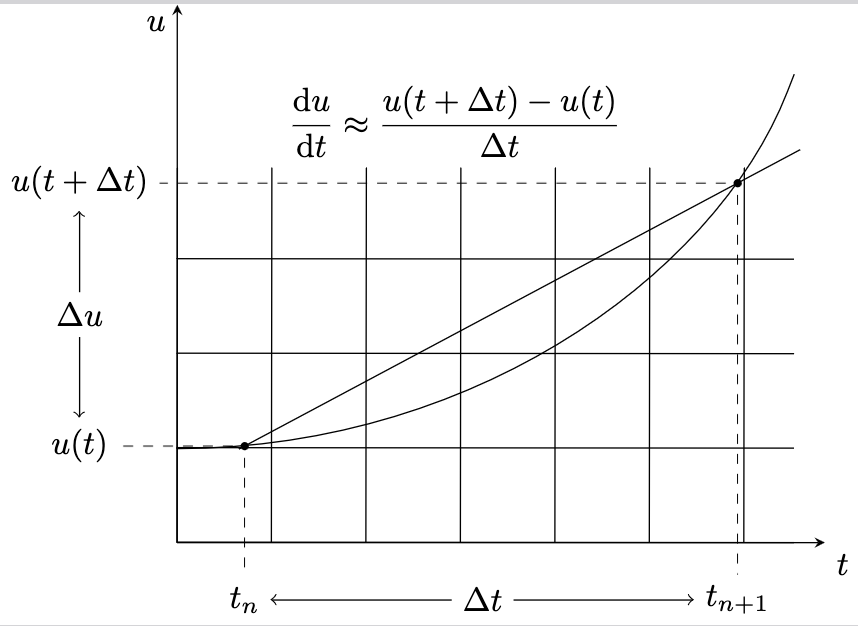
\includegraphics[height=120pt]{papers/spektral/images/forwarddiff.png}
	\caption{Vorwartsdifferenz}
    \label{spektral:fig:gittermodelle}
\end{figure}

Auf der Abbildung 16.1 sieht man, dass für eine 1d-Funktion werden viele Punkte für die Vorheraussage benötigt. In der 3-Dimensionen es sind die Millionen von Datenpunkten und, damit man eine gute Wetterprognose mit der Methode machen kann, werden höhe Rechnungsleistungen benötigt.

Ein Optimierung ist, die Prognosenfunktion auf eine andere Art zu aproximieren.

\subsection{Was sind die spektrale Modelle?
\label{spektral:subsection:spektralemodelle}}
In den 1980er Jahren des 20. Jahrhunderts wurden neben den gitterbasierten (Finite-Difference) Lösungsmethoden, die traditionell in Vorhersagemodellen verwendet wurden, auch Methoden angewendet, bei denen die räumliche Abhängigkeit der prognostizierten meteorologischen Werten als Reihen von Funktionssystemen dargestellt wird, die bestimmte Eigenschaften aufweisen.

In diesem Fall wird die prognostizierte Gleichung oder das System von partiellen Differentialgleichungen auf Systeme von Differentialgleichungen für die zeitabhängigen Koeffizienten der Zerlegung reduziert.
Die gesuchte Werte bei diesem Ansatz sind diese Koeffizienten und nicht die Werte der prognostizierten Funktionen an den Gitterpunkten. 
Eine Variante dieser Methode im Bereich der numerischen Wettervorhersage wird als spektrale Methode bezeichnet und Vorhersagemodelle, bei denen die Gleichungen mit der spektralen Methode gelöst werden, werden als spektrale Modelle bezeichnet.

Spektrale Modelle sind eine Art numerischer Modelle, die in verschiedenen wissenschaftlichen Bereichen, einschließlich der Meteorologie, verwendet werden.
Diese Modelle basieren auf der Verwendung spektraler Methoden, um mathematische Gleichungen, die physikalische Phänomene beschreiben, zu lösen.

In der Meteorologie beziehen sich spektrale Modelle auf Vorhersagemodelle, die spektrale Methoden verwenden, um atmosphärische Prozesse zu simulieren und Wettervorhersagen zu erstellen.
Anstatt die Erde und die Atmosphäre in einem diskreten Gitter zu modellieren, wie es bei gitterbasierten Modellen der Fall ist, verwenden spektrale Modelle eine Fourier-Transformation, um die Atmosphäre in eine Kombination von Wellen mit verschiedenen Frequenzen aufzubrechen.
Dies ermöglicht es, die Atmosphäre kontinuierlich und mit höherer Auflösung zu modellieren.

Insgesamt sind spektrale Modelle ein wichtiger Ansatz, um detaillierte Einblicke in atmosphärische Prozesse zu gewinnen und präzise Wettervorhersagen zu erstellen, insbesondere wenn es um die Wellen und die Schwingungen geht.

\subsection{Vorteile der spektralen Modellen
\label{spektral:subsection:vorteile}}

\begin{itemize}
\item
\textbf{Genauere Erfassung von Wellenphänomenen:} Spektrale Modelle sind besonders gut darin, atmosphärische Wellenphänomene wie Schallwellen, Rossby-Wellen und atmosphärische Oszillationen zu erfassen.
Sie können die räumliche Ausbreitung und Interaktion dieser Wellen genau simulieren.
\item
\textbf{Bessere Darstellung von großen und kleinen Skalen:} Spektrale Modelle haben eine hohe räumliche Auflösung, die es ermöglicht, sowohl großräumige globale Muster als auch kleinräumige lokale Effekte detailliert zu modellieren.
Dadurch können sie sowohl makroskalige als auch mikroskalige Phänomene abdecken.
\item
\textbf{Konsistente Erhaltung bestimmter Größen:} Spektrale Modelle haben oft eine bessere Erhaltung von Energie, Impuls und anderen wichtigen physikalischen Größen.
Dies trägt zur Erzielung physikalisch konsistenterer Simulationen bei.
\item
\textbf{Effiziente Modellierung periodischer Phänomene:} Spektrale Modelle sind gut geeignet zur Modellierung periodischer Phänomene, da sie periodische Signale genau erfassen können, ohne hohe räumliche Auflösung überall zu erfordern.
\item
\textbf{Reduzierter Diffusionseffekt (Rauschen resistent):} Im Vergleich zu einigen gitterbasierten Methoden, die zur Stabilisierung numerischer Instabilitäten künstliche Diffusion einführen müssen, weisen spektrale Modelle oft einen geringeren Diffusionseffekt auf, was zu genaueren und detaillierteren Simulationen führen kann.
\item
\textbf{Adaptivität und Flexibilität:} Spektrale Modelle können auf verschiedene Geometrien und Randbedingungen angewendet werden und sind nicht auf regelmäßige Gitterstrukturen beschränkt. Dies ermöglicht eine höhere Anpassungsfähigkeit an komplexe Geländeformen.
\item
\textbf{Einfachere Lösung:} Spektralen Modellen führen auf viel einfache algebraische Gleichungen.
\end{itemize}

\subsection{Kugelkoordinaten
\label{spektral:subsection:kugelkoordinaten}}

Bevor wir die spektrale Modelle nähe anschauen, müssen wir die von den kartesischen Koordinaten zu den Kugelkkordinaten wecheln, weil wir uns auf einer Kugel befinden. Siehe Abbildung 16.2

\begin{figure}[h]
	\centering
	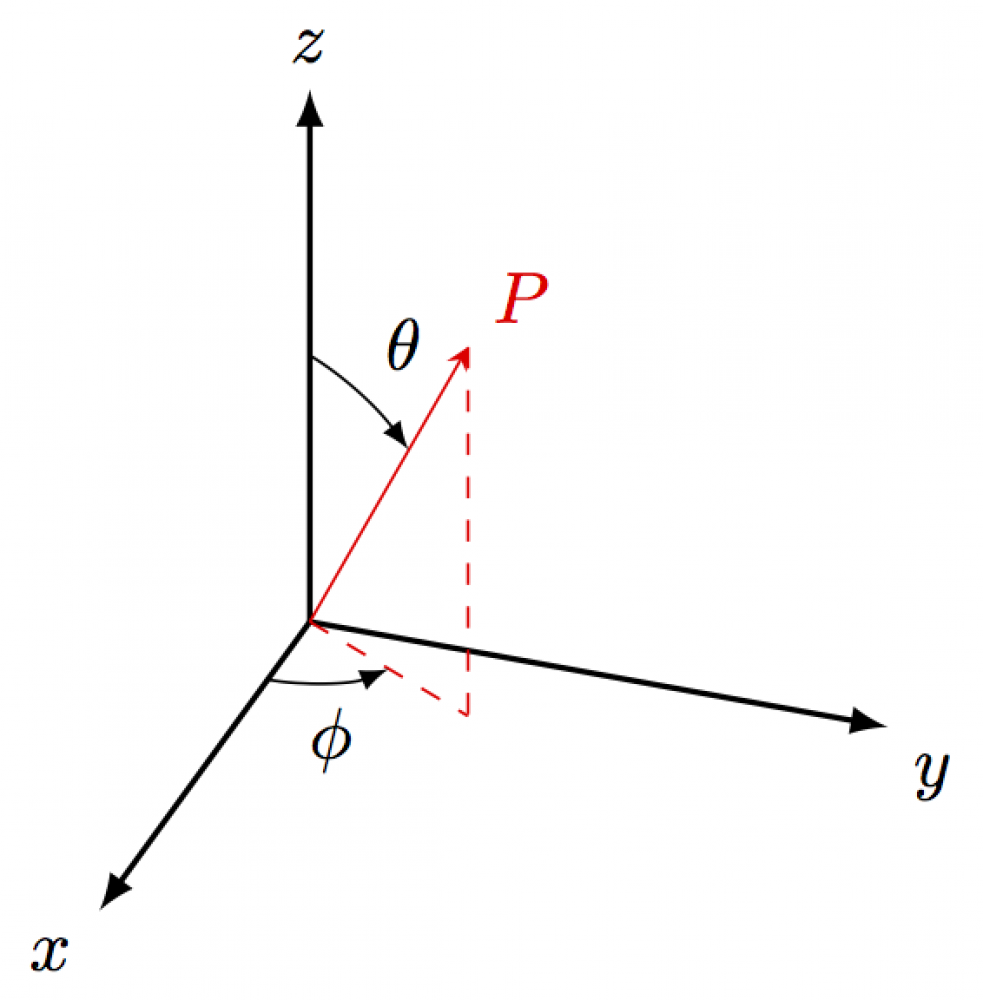
\includegraphics[height=120pt,width=120pt]{papers/spektral/images/spherical_coordinates.png}
	\caption{Sphärische Koordinaten}
    \label{spektral:fig:sphericalcoords}
\end{figure}
\pagebreak
\begin{equation}
 x = r*\sin(\theta)*\cos(\phi)
\label{spektral:equation4}
\end{equation}

\begin{equation}
 y = r*\sin(\theta)*\sin(\phi)
\label{spektral:equation5}
\end{equation}

\begin{equation}
 z = r*\cos(\theta)
\label{spektral:equation6}
\end{equation}
wobei |r| > 0 sein muss, sonst können $\theta$ und $\phi$ nicht definiert werden.



%
% Spektrale Modelle.tex -- Beispiel-File für teil2 
%
% (c) 2023 Dmitry Grigoriev, OST Ostschweizer Fachhochschule
%
% !TEX root = ../../buch.tex
% !TEX encoding = UTF-8
%
\section{Spektrale Modelle 
\label{spektral:section:spektralemodelle}}
\rhead{Spektrale Modelle}

Wir werden die Idee der Spektralmethode auf einem Beispiel anschauen. Dafür nehmen wir die Wellengleichung

\begin{equation}
 \dfrac{\partial^2U}{\partial{t^2}} = \alpha^2\Delta{U}.
\label{spektral:equation7}
\end{equation}
Durch eine sehr aufwändige Rechnung, kann die Wellengleichung in den Kugelkoordinaten folgendermaßen geschrieben werden (siehe \cite[Anhang B]{spektral:QuantenmechanikMathemathischesSeminar}):

\begin{equation}
 \frac{1}{r^2}\frac{\partial}{\partial{r}}\left(r^2\frac{\partial{U}}{\partial{r}}\right) + \frac{1}{r^2}\left(\frac{1}{\sin\theta}\frac{\partial}{\partial{\theta}}\left(\sin\theta\frac{\partial{U}}{\partial{\theta}}\right) + \frac{1}{\sin^2\theta}\frac{\partial^2{U}}{\partial{\phi^2}}\right) = \frac{1}{\alpha^2}\frac{\partial^2{U}}{\partial{t^2}}.
\label{spektral:equation8}
\end{equation}
Diese Gleichung ist sehr schwer zu lösen und bei der Lösung werden uns die spektrale Modelle helfen.

\subsection{Kugelflächenfunktionen
\label{spektral:subsection:kugelflaechenfunktionen}}

Damit wir das spektrale Modell für die Gleichung \eqref{spektral:equation7} entwicklen können, werden wir ein vollständigen und orthogonaler Satz von Basisfunktionen benötigt.
Dafür muss die Eigenwertgleichung des Laplace-Operators \eqref{spektral:equation8}

\begin{equation}
 \Delta{V} = -\lambda{V(x)}
\label{spektral:equation9}
\end{equation}
gelöst werden.
Die vollständige Lösung ist in \cite[Seite 62]{spektral:NichtkommutativeBildvearbeitung} gezeigt.
Für uns ist wichtig, dass wir die Basisfunktionen finden und durch diese Funktionen --- Kugelflächenfunktionen (siehe \cite{spektral:MathsemSpezfunk} und \cite{spektral:NichtkommutativeBildvearbeitung}) --- unsere gesuchte Funktion aus der Gleichung \eqref{spektral:equation7} als

\begin{equation}
u(\phi,\theta,t) = \sum_{m=0}^{\infty}\sum_{n=-m}^{\infty}a_n^m(t)Y_n^m(\phi, \theta)
\label{spektral:equation10}
\end{equation}
darstellen können.

\subsection{Wellengleichung
\label{spektral:subsection:wellengleichung}}
Jetzt sind wir bereit die Wellengleichung mit der spektrale Methode zu lösen.
Für die Vereinfachung nehmen wir an, dass in der Gleichung \eqref{spektral:equation7} $\alpha=1$ ist und der Kugelradius auch $r=1$ ist.
Dann wird die Wellengleichung so aussehen:
\begin{equation}
\frac{1}{\sin\theta}\frac{\partial}{\partial{\theta}}\left(\sin\theta\frac{\partial{U}}{\partial{\theta}}\right) + \frac{1}{\sin^2\theta}\frac{\partial^2{U}}{\partial{\phi^2}} = \frac{\partial^2{U}}{\partial{t^2}}.
\label{spektral:equation11}
\end{equation}
Wenn wir die Gleichung \eqref{spektral:equation10} für die Gleichung \eqref{spektral:equation7} anwenden, dann bekommen wir
\begin{equation}
\Delta{U} = \sum_{m=0}^{\infty}\sum_{n=-m}^{\infty}a_n^m(t)\Delta{Y_n^m(\phi, \theta)}.
\label{spektral:equation12}
\end{equation}
Wir müssen jetzt die $\Delta{Y_n^m(\phi, \theta)}$ finden.
Das können wir aus den Laplace-Operator in sphärischen Koordinaten ausrechnen. Wir wissen, dass der Laplace-Operator selbstadjungiert ist, seine Eigenfunktionen orthogonal sind und der Eigenwert $-l(l+1)$ ist (siehe Satz~\ref{buch:orthofkt:pde:satz:kugel}).
Diese Information erlaubt uns die harmonisches Analysis durchzuführen.
Gemäß dem Satz~\ref{buch:orthofkt:pde:satz:kugel} bekommen wir
\begin{equation}
\Delta{Y_n^m(\phi, \theta)} = -l(l+1)Y_n^m(\phi, \theta).
\label{spektral:equation16}
\end{equation}
Laplace-Operator der Kugelflächenfunktion ist proportional der Funktion selbst \cite[Seite 663]{spektral:DynamicOfTheAtmosphere}. Das ist sehr wichtige Eigenschaft, die wir gleich anwenden werden.
Aus der Gleichung \eqref{spektral:equation12} bekommen wir:
\begin{equation}
\Delta{U} = -\sum_{m=0}^{\infty}\sum_{n=-m}^{\infty}a_n^m(t)l(l+1)Y_n^m(\phi, \theta)
\label{spektral:equation17}
\end{equation}
und wenn wir die Gleichung \eqref{spektral:equation10} auf die linke Seite der Gleichung \eqref{spektral:equation7} anwenden, bekommen wir
\begin{equation}
\sum_{m=0}^{\infty}\sum_{n=-m}^{\infty}\ddot{a}_n^m(t)Y_n^m(\phi, \theta) = -\sum_{m=0}^{\infty}\sum_{n=-m}^{\infty}a_n^m(t)l(l+1)Y_n^m(\phi, \theta).
\label{spektral:equation18}
\end{equation}
Wir stellen fest, dass auf den beiden Seiten der Gleichung die Kugelflächenfunktion $Y_n^m(\phi, \theta)$ vorkommt, und die Gleichung \eqref{spektral:equation18} kann in 
\begin{equation}
\ddot{a}_n^m(t) = -l(l+1)a_n^m(t)
\label{spektral:equation19}
\end{equation}
umgeschrieben werden.
Dadurch bekommen wir ein System der Differenzialgleichungen zweiter Ordnung, das folgende Lösungen hat:
\begin{equation}
a_n^m(t) = a_n^m(0)e^{i\sqrt{l(l+1)}t}.
\label{spektral:equation20}
\end{equation}
Somit die gesuchte Funktion ist
\begin{equation}
u(\phi, \theta, t) = \sum_{m=0}^{\infty}\sum_{n=-m}^{\infty}a_n^m(0)e^{i\sqrt{l(l+1)}t}Y_n^m(\phi, \theta).
\label{spektral:equation21}
\end{equation}

\subsection{Ergebnis
\label{spektral:subsection:ergebnis}}

Als Ergebnis bekommen wir die Gleichung, die im Vergleich zu Differenzialgleichung \eqref{spektral:equation8} wesentlich einfacher zu lösen ist.
Dieser Vorteil wurde bereits im Abschnitt \ref{spektral:subsection:vorteile} erwähnt und wurde nun bestätigt.
%
% Spektrale Modelle.tex -- Beispiel-File für teil2 
%
% (c) 2023 Dmitry Grigoriev, OST Ostschweizer Fachhochschule
%
% !TEX root = ../../buch.tex
% !TEX encoding = UTF-8
%
\section{Meteorologische Modelle in der Wettervorhersage
\label{spektral:section:modelle}}
\rhead{Meteorologische Modelle}

Im Oktober 1973 wurde das Europäische Zentrum für mittelfristige Wettervorhersage (EZMW) gegründet \cite{spektral:ezmw} und hat die erste Vorhersagen am 1. August 1979 publiziert.
Seit 1979 sind die Wetterprognosen, dank der spektralen Modelle, viel besser geworden.

Heute haben wir fast unendliche Rechenleistung zur Verfügung (z.B. Cloud-Computing), aber wir müssen trotzdem unsere Reihe \eqref{spektral:equation21} an eine fixe Anzahl der Wellen $(N)$ begrenzen.
In der echten Welt wird die Gleichung \eqref{spektral:equation21} so aussehen:
\begin{equation}
u(\phi, \theta, t) = \sum_{m=-0}^{N}\sum_{n=-m}^{m}a_n^m(0)e^{i\sqrt{l(l+1)}t}Y_n^m(\phi, \theta).
\label{spektral:equation22}
\end{equation}
$N$ wird Modelauflösung genannt \cite[Seite 223]{spektral:NumericalWeatherPrediction} und \eqref{spektral:equation21} als \textit{Dreieickabschneidung} (triangular truncation) genannt.
Z.B: wenn das Model $N = 512$ hat, dann wird das Model T512 bezeichnet. 
Im Frühjahr 2006 wurden die Modelle aktualisiert. Das determinischte Model heißt jetzt T799 (vorher T511) \cite[Seite 222]{spektral:NumericalWeatherPrediction}.
\begin{figure}[h]
	\centering
	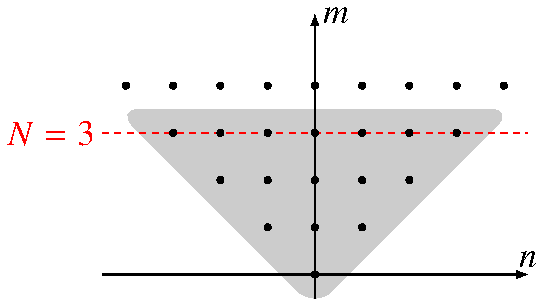
\includegraphics[height=140pt]{papers/spektral/images/triangle_truncation.pdf}
	\caption{Dreieickabschneidung}
    \label{spektral:fig:triangletrunc}
\end{figure}

Abschließend lässt sich festhalten, dass die Anwendung spektraler Modelle in der Meteorologie einen bedeutenden Fortschritt in der Erforschung und Vorhersage atmosphärischer Phänomene darstellt.
Diese Modelle ermöglichen es, komplexe Prozesse in der Atmosphäre auf einer spektralen Ebene zu analysieren und somit tiefgreifendes Verständnis zu erlangen.
Die Nutzung von spektralen Modellen hat maßgeblich zur Verbesserung der Genauigkeit von Wettervorhersagen beigetragen und ermöglicht gleichzeitig Einblicke in langfristige Klimatrends.
Doch trotz dieser Fortschritte stehen auch weiterhin Herausforderungen wie die Feinabstimmung der Modelle und die Berücksichtigung aller relevanten Faktoren.
Während wir uns in eine Ära fortschrittlicher Technologien begeben, werden spektrale Modelle zweifellos weiterhin eine Schlüsselrolle bei der Entschlüsselung der Geheimnisse unseres Wetters und Klimas spielen.


\printbibliography[heading=subbibliography]
\end{refsection}
